\section{Глава 1. Название главы}
\subsection{Операции над множествами.}

\begin{enumerate}
    \item Объединение 
      \[A \cup B=\{x|x \in A \lor x\in B\}\]
    \begin{center}   
      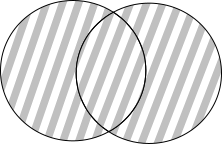
\includegraphics[scale=0.65]{bitmap.png}
    \end{center}
  \end{enumerate}

\subsection{Понятие класса.}

Класс - чертеж объекта, основа из чего будет создаваться объект. Определяет какие атрибуты и методы будут принадлежать все его объектам.

\begin{lstlisting}
public class ClassTwo {
    private String name;

    public String getName() {
        return name;
    }
 
    public void setName(String name) {
        this.name = name;
    } 
}

\end{lstlisting}